\documentclass[tikz]{standalone}
% \usetikzlibrary{intersections}
\usetikzlibrary{angles}
\date{}
\usepackage{amsmath,amsthm,amssymb}
\usepackage{xcolor}
\usepackage{tikz}
\usepackage[siunitx]{circuitikz}
\usepackage{tikz-3dplot}
\usepackage{ifthen}
\tikzset{isometricXYZ/.style={x={(-0.866cm,-0.5cm)}, y={(0.866cm,-0.5cm)}, z={(0cm,1cm)}}}
\usetikzlibrary{arrows,decorations.pathmorphing,positioning,fit,trees,shapes,automata,calc,intersections,decorations.markings,patterns,graphs,quotes,plotmarks}
%\usepackage{algorithm}
%\usepackage{algorithmic}
\newcommand{\R}{\mathbb{R}}
\newcommand{\F}{\mathbb{F}}
\newcommand{\bmat}[1]{\begin{bmatrix}#1\end{bmatrix}}
\newcommand{\xth}[1]{{#1}^{\mathrm{th}}}
\newcommand{\pd}[2]{\frac{\partial #1}{\partial #2} }
\newcommand{\pdd}[2]{\frac{\partial^2 #1}{\partial #2^2}}
\newcommand{\myitemsep}{\setlength\itemsep{-0.25em}}
\newcommand{\bigpar}[1]{\left( #1\right)}
\tikzset{myedge/.style={ thick,->,>=stealth',inner sep=0pt,outer sep=3pt}}
\tikzset{hv path/.style= {to path={-| (\tikztotarget)}}}
\tikzset{vh path/.style= {to path={|- (\tikztotarget)}}}

%%%%%%%%%% Using shift and rotate around:

\newcommand{\spring}[4]{
\path[shift={#1},rotate={#2},fill = white,opacity=1.0] (-0.25,-0.5) rectangle (0.25,0.5); % cover
\draw[thick,shift={#1},rotate={#2}] (0,0.5) -- +(0.25,-0.1) -- +(-0.25,-0.2)-- +(0.25,-0.3)-- +(-0.25,-0.4)-- +(0.25,-0.5)-- +(-0.25,-0.6)-- +(0.25,-0.7)-- +(-0.25,-0.8)-- +(0.25,-0.9) -- +(0,-1.0);
\draw[thick,shift={#1},rotate={#2}] (#3,0) node {#4};
}
\newcommand{\ground}[3]{
\draw[thick,shift={#1},rotate={#2}] (-0.5*#3cm,0) -- (0.5*#3cm,0);
\path[thick,shift={#1},rotate={#2},pattern=north west lines] (-0.5*#3cm,0) rectangle (0.5*#3cm,0.2);
}
\newcommand{\dashpot}[4]{
\path[shift={#1},rotate={#1},fill = white,opacity=1.0] (-0.25,0) rectangle (0.25,0.15);
\path[shift={#1},rotate={#1},draw,thick] (0,0) -- +(0.25,0) -- +(0.25,0.25) +(0.15,0.15) -- +(-0.15,0.15)  +(-0.25,0.25) -- +(-0.25,0) -- +(0,0);
\draw[thick,shift={#1},rotate={#1}] (#3,0) node {#4};
}
\newcommand{\mydashpot}[5]{
\begin{scope}[xshift=#1cm,yshift=#2cm,rotate=#3]
	\path[fill = white,opacity=1.0] (-0.25,0) rectangle (0.25,0.15);
	\path[draw,thick] (0,0) -- +(0.25,0) -- +(0.25,0.25) +(0.15,0.15) -- +(-0.15,0.15)  +(-0.25,0.25) -- +(-0.25,0) -- +(0,0);
	\node at (#4,0) {#5};
	\end{scope}
}
\newcommand{\lapof}[1]{\mathcal L \left\{ #1 \right\}}
\newcommand{\lapinv}[1]{\mathcal L^{-1} \left\{ #1 \right\}}
\newcommand{\evalat}[2]{\left. #1 \right|_{#2}}
\newcommand{\myarr}[3]{(-#2:#1) arc (-#2:#2:#1) node[#3] }
\newcommand{\mc}[1]{\mathcal{#1}}
\newcommand{\mred}[1]{\textcolor{red}{[#1]}}
\newcommand{\myco}[2]{\bigpar{ \frac{#1}{#2} }}
\newcommand{\tc}[2]{{#1}{#2}}
\newcommand{\mcb}[1]{{\color{blue}#1}}
\newcommand{\mcr}[1]{{\color{red}#1}}
\newcommand{\mcg}[1]{{\color{green!70!black}#1}}
\usepackage{hyperref}
\hypersetup{colorlinks=true,
linkcolor=blue,          % color of internal links
        citecolor=green,        % color of links to bibliography
          filecolor=magenta,      % color of file links
           urlcolor=blue           % color of external links
}


\begin{document}
\tikzset{help lines/.style=very thin}
\tikzset{Karl's grid/.style={help lines,color=blue!50}}

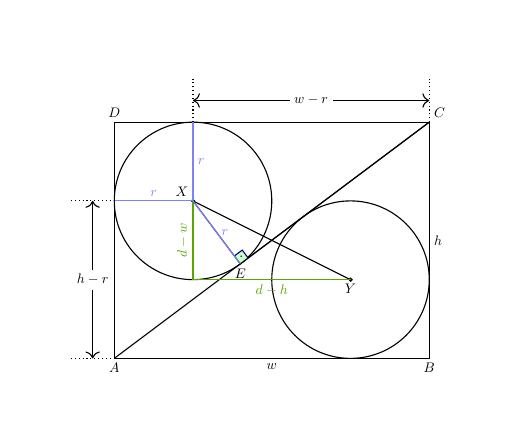
\begin{tikzpicture}[every node/.style={scale=0.5}]
  \clip (-1.1,-0.5) rectangle (4.8,4.2);
  \draw[thin] (0,0) rectangle (4,3);
  \draw (0,0) -- (4,3);
  \draw (1.0, 2.0) circle [radius=1cm];
  \draw (3.0, 1.0) circle [radius=1cm];
  \draw (1.0, 2.0) -- (3.0, 1.0);
  \filldraw (1.0, 2.0) circle [radius=0.2mm];
  \filldraw (3.0, 1.0) circle [radius=0.2mm];
  \draw (1.0,2.0) node[above left] {$X$};
  \draw (3.0,1.0) node[below] {$Y$};
  \draw (2.0,0.0) node[below] {$w$};
  \draw (4.0,1.5) node[right] {$h$};

  \draw[color=blue!50] (1.0,2) -- node[right] {$r$} (1.0,3);
  \draw[color=blue!50] (1.0,2) -- node[above] {$r$} (0.0,2);


  \draw[densely dotted] (-0.55,{3-1.0}) -- (0,{3-1});

  \draw[densely dotted] (-0.55,{0}) -- (0,0);
  \draw[<->] (-0.275,{0}) -- node[fill=white]{$h-r$} (-0.275,2);

  \draw[densely dotted] (1.0,3) -- (1.0,3.55);
  \draw[densely dotted] (4.0,3) -- (4.0,3.55);
  \draw[<->] (1.0,3.275) -- node[fill=white]{$w-r$} (4.0,3.275);

  \draw[color=green!65!red] (1.0,2.0) -- node[above, rotate=90]{$d-w$}(1.0,1.0);
  \draw[color=green!65!red] (1.0,1.0) -- node[below]{$d-h$} (3.0,1.0);


  \coordinate (A) at (0,0);
  \coordinate (B) at (4,0);
  \coordinate (C) at (4,3);
  \coordinate (D) at (0,3);
  \coordinate (E) at (1.6,1.2);
  \coordinate (X) at (1.0,2.0);

  \draw (A) node[below] {$A$};
  \draw (B) node[below] {$B$};
  \draw (C) node[above right] {$C$};
  \draw (D) node[above] {$D$};
  \draw (E) node[below] {$E$};

  \draw (C) -- (E) -- (X) pic [draw=blue!50!black, fill=green!20, 
          scale=0.5, angle eccentricity=.5, pic text=.] {right angle = C--E--X};
  \draw[color=blue!50, xshift=1cm, yshift=2cm, rotate=-53.13010235415598] (0,0)
          -- node[right] {$r$} (1.0,0.0);
\end{tikzpicture}

\end{document}
